%%%%%%%%%%%%%%%%%%%%%%%%%%%%%%%%%%%%%%%%%%%%%%%%%%%%%%%%%%%%%%%%%%%%%%%%%%%%%%%%%%%%%%%%%%%%%%%%%%%%%%%%%%%%%%%%%%%%%%%%%%%%%%%%%%%%%%%%%%%%%%%
%%%%%%%%%%%%%%%%%%%%%%%%%%%%%%%%%%%%%%%%%%%%%%%%%%%%%%%%%%%%%%%%%%%%%%%%%%%%%%%%%%%%%%%%%%%%%%%%%%%%%%%%%%%%%%%%%%%%%%%%%%%%%%%%%%%%%%%%%%%%%%%
\section{Hardware}
\label{sec:Hardware}
%%%%%%%%%%%%%%%%%%%%%%%%%%%%%%%%%%%%%%%%%%%%%%%%%%%%%%%%%%%%%%%%%%%%%%%%%%%%%%%%%%%%%%%%%%%%%%%%%%%%%%%%%%%%%%%%%%%%%%%%%%%%%%%%%%%%%%%%%%%%%%%
%%%%%%%%%%%%%%%%%%%%%%%%%%%%%%%%%%%%%%%%%%%%%%%%%%%%%%%%%%%%%%%%%%%%%%%%%%%%%%%%%%%%%%%%%%%%%%%%%%%%%%%%%%%%%%%%%%%%%%%%%%%%%%%%%%%%%%%%%%%%%%%

This section introduces the new magnetic fiducial tags (MFTags) which are implemented on the 3D M-Block Modules~\cite{Romanishin20153d}. Basic information regarding 3D M-Blocks is presented in Table~\ref{tab:hardwareOverviewTable}. These modules can pivot on a cubic lattice using pulses of angular momentum from an internal reaction wheel according to the pivoting cube model.
%%%%%%%%%%%%%%%%%%%%%%%%%%%%%%%%%%%%%%%%%%%%%%%%%%%%%%%%%%%%%%%%%%%%%%%%%%%%%%%%%%%%%%%%%%%%%%%%%%%%%%%%%%%%%%%%%%%%%%%%%%%%%%%%%%%%%%%%%%%%%%%
%%%%%%%%%%%%%%%%%%%%%%%%%%%%%%%%%%%%%%%%%%%%%%%%%%%%%%%%%%%%%%%%%%%%%%%%%%%%%%%%%%%%%%%%%%%%%%%%%%%%%%%%%%%%%%%%%%%%%%%%%%%%%%%%%%%%%%%%%%%%%%%
\begin{table}[h]
	\caption{Basic characteristics of the 3D M-Blocks robotic platform modules.}
	\centering
	\begin{tabular}{ p{3.5cm}  p{2cm} }
		\hline
		Actuation Directions & 6 \\
		Mass  & 163\,g \\
		Characterist Dimension & 50\,mm \\
		Total Parts  & 216 \\
	%	Number fabricated  & 16 \\
	%	Est. Cost & \$230 \\
	\end{tabular}
	\label{tab:hardwareOverviewTable}
\end{table}
%%%%%%%%%%%%%%%%%%%%%%%%%%%%%%%%%%%%%%%%%%%%%%%%%%%%%%%%%%%%%%%%%%%%%%%%%%%%%%%%%%%%%%%%%%%%%%%%%%%%%%%%%%%%%%%%%%%%%%%%%%%%%%%%%%%%%%%%%%%%%%%
%%%%%%%%%%%%%%%%%%%%%%%%%%%%%%%%%%%%%%%%%%%%%%%%%%%%%%%%%%%%%%%%%%%%%%%%%%%%%%%%%%%%%%%%%%%%%%%%%%%%%%%%%%%%%%%%%%%%%%%%%%%%%%%%%%%%%%%%%%%%%%%

In order to add neighbor detection and connection orientation functionality to the 3D M-Blocks this section introduces the \TagNamePlural, which is a new fiducial tag system which allows modules to detect information about their neighbors through magnetic fields, and is shown in Figure~\ref{fig:tagDiagram}. The following design criteria were taken into consideration while creating \TagNamePlural, specifically that they should be able to:
\begin{itemize}
	\item \emph{be read passively} - information can be read even when the module is inactive.
	\item \emph{be fabricated inexpensively} - necessary for scaling systems of beyond 1000 of modules.
	\item \emph{identify many unique ID's} - needs to provide accurate ID information for significant number of tags in large systems.
	\item \emph{detect connector orientations} - the tag needs to reliably determine the 90-degree angle of the tag relative to the reader.
\end{itemize} 

\TagNamePlural~are essentially specific arrangements of permanent magnets mounted on the connectors of each modules.  The orientation of the magnets which comprise a \tagName~can be measured by simple absolute magnetic encoder ICs, thereby reading information encoded in the orientation of the magnets, and encoding information. Detecting the angle of the magnets is accomplished through using an absolute on-axis magnetic encoder IC. Each active module has been outfitted with a circuit board that includes two Austrian Microsystems AS5048B absolute magnetic encoders, a light sensor, and several LEDs. The circuit boards are driven from the central processor through an I2C I/O expander.

%%%%%%%%%%%%%%%%%%%%%%%%%%%%%%%%%%%%%%%%%%%%%%%%%%%%%%%%%%%%%%%%%%%%%%%%%%%%%%%%%%%%%%%%%%%%%%%%%%%%%%%%%%%%%%%%%%%%%%%%%%%%%%%%%%%%%%%%%%%%%%%
%%%%%%%%%%%%%%%%%%%%%%%%%%%%%%%%%%%%%%%%%%%%%%%%%%%%%%%%%%%%%%%%%%%%%%%%%%%%%%%%%%%%%%%%%%%%%%%%%%%%%%%%%%%%%%%%%%%%%%%%%%%%%%%%%%%%%%%%%%%%%%%
\begin{table}[b]
	\caption{Information content in the \TagNamePlural~encoding specification. The current system is limited to 2 angle sensors due to practical considerations of the physical dimensions of the  PCBa's in the 3D M-Blocks. Extending the reader to include  four sensors would increase the number of unique tags by over 300 times.}
	
	\begin{tabular}{ p{1.6cm}  p{1.8cm}  p{1.9cm}  p{1.5cm}}
		\hline
								& \textit{Current system} & Future extension & Extended \\
		\hline
				\addlinespace[1ex]
		Magnets  				& 4 			 &	4				&	4	\\
		Digits 					& 30 			 &	24				&	48	\\
		\# Of Sensors 			& 2 			 &	4				&	4	\\
		\textit{Unique Tags} 	& \textbf{900} 	 & 331776			& 	~5,000,000\\
		
	\end{tabular}
	
	\label{tab:hardwareOverview}
\end{table}
%%%%%%%%%%%%%%%%%%%%%%%%%%%%%%%%%%%%%%%%%%%%%%%%%%%%%%%%%%%%%%%%%%%%%%%%%%%%%%%%%%%%%%%%%%%%%%%%%%%%%%%%%%%%%%%%%%%%%%%%%%%%%%%%%%%%%%%%%%%%%%%
%%%%%%%%%%%%%%%%%%%%%%%%%%%%%%%%%%%%%%%%%%%%%%%%%%%%%%%%%%%%%%%%%%%%%%%%%%%%%%%%%%%%%%%%%%%%%%%%%%%%%%%%%%%%%%%%%%%%%%%%%%%%%%%%%%%%%%%%%%%%%%%

The underlying hypothesis is that low cost and lack of RF transmission make magnets an attractive choice for a technology that may have to be implemented thousands of times in a set of reconfigurable modules. The ability to use several such sensors at close proximity prevents interference between reading faces, while still providing enough data to read tag orientation as well as a unique identity. The \tagNamePlural~were designed and tested with the 3D M-Blocks modular robots as the test bed, although nothing precludes their use in other systems.

%%%%%%%%%%%%%%%%%%%%%%%%%%%%%%%%%%%%%%%%%%%%%%%%%%%%%%%%%%%%%%%%%%%%%%%%%%%%%%%%%%%%%%%%%%%%%%%%%%%%%%%%%%%%%%%%%%%%%%%%%%%%%%%%%%%%%%%%%%%%%%%
%%%%%%%%%%%%%%%%%%%%%%%%%%%%%%%%%%%%%%%%%%%%%%%%%%%%%%%%%%%%%%%%%%%%%%%%%%%%%%%%%%%%%%%%%%%%%%%%%%%%%%%%%%%%%%%%%%%%%%%%%%%%%%%%%%%%%%%%%%%%%%%
%%%%%%%%%%%%%%%%%%%%%%%%%%%%%%%%%%%%%%%%%%%%%%%%%%%%%%%%%%%%%%%%%%%%%%%%%%%%%%%%%%%%%%%%%%%%%%%%%%%%%%%%%%%%%%%%%%%%%%%%%%%%%%%%%%%%%%%%%%%%%%%
%%%%%%%%%%%%%%%%%%%%%%%%%%%%%%%%%%%%%%%%%%%%%%%%%%%%%%%%%%%%%%%%%%%%%%%%%%%%%%%%%%%%%%%%%%%%%%%%%%%%%%%%%%%%%%%%%%%%%%%%%%%%%%%%%%%%%%%%%%%%%%%
\begin{figure*}[th]
	
	\newsavebox{\faceDiagram}
	\sbox{\faceDiagram}	{
		\newcommand{\statcirc}[4]{
	\fill[opacity = 0.5, red,shift={(#1 cm,#2 cm)}, rotate=#3] (0,0) circle (#4); 
	\fill[opacity = 0.5, blue,shift={(#1 cm,#2 cm)},rotate=#3] (0,0) -- (180:#4) arc (180:0:#4) -- cycle;
	%	\draw[->,black,shift={(#1 cm,#2 cm)},rotate=#3] (#4, 0)
}

\newcommand{\drawArrow}[3]{
	\draw[->,>={Stealth[round]}, line width=0.75mm, black ,shift={(#1 cm,#2 cm)}, rotate=#3] (0,-0.5) -- (0,0.5); 
}

\newcommand{\drawchip}[3]{
	\tikzmath
	{
		\chipW = 0.35;
		\chipH = 0.4;
	}
	\fill[opacity = 0.75, darkgray, shift= {(#1 cm, #2 cm)}, rotate = #3, rounded corners] (-\chipH,-\chipW) rectangle (\chipH,\chipW);
	\fill[orange,shift= {(#1 cm, #2 cm)}, rotate = #3 ] (-0.25,0.2) circle (0.1);
}
\begin{tikzpicture}

	\tikzmath{
		\offsetAxis = 0.5;
		\offsetCent = 2.9;
		\diameter = 0.32;
	}
	\draw node (A) at (-0.5, 1.7) {};
	\draw node (B) at (0, 1.7) {};
	\drawchip{\offsetAxis}{\offsetCent}{0};
	\drawchip{-\offsetAxis}{-\offsetCent}{180};
	
	%Magnet North
	\statcirc{-\offsetAxis}{\offsetCent}{70}{\diameter};
	
	\drawArrow{-\offsetAxis}{\offsetCent}{70}
	
	%Magnet EAST
	\statcirc{\offsetCent}{\offsetAxis}{20}{\diameter};
	
	% Magnet West
	\statcirc{\offsetAxis}{-\offsetCent}{190}{\diameter};
	
	\statcirc{-\offsetCent}{-\offsetAxis}{45}{\diameter};
	
	\draw[gray, dashed] (-\offsetAxis,{\offsetCent + 1}) -- 
	(-\offsetAxis,{\offsetCent - 1});
	\draw[black,dotted] (0,0) circle (2.95);
	
	% 4 Cross Lines X
	\draw[black,dashed] (0,0) -- (4,0);
	\draw[black,dashed] (0,0) -- (-4,0);
	\draw[black,dashed] (0,0) -- (0,4);
	\draw[black,dashed] (0,0) -- (0,-4);
	
%	\draw[purple, dotted] ()
	% Dimensioned Variables
	\dimline[line style = {line width = 0.8, arrows = dimline reverse-dimline reverse}] {(A)}{(B)}{x};
	
	% Arc Radius
	\dimline[line style = {line width = 0.8}] {(0,0)} {++(150:2.95)}{R};
%	\dimline {(1,0)}{(-1,0)}{x};
\end{tikzpicture}
	}
	
	\newsavebox{\magnetDigitization}
	\sbox{\magnetDigitization}	{
		
\newcommand{\statcirc}[4]{
	\fill[red,shift={(#1 cm,#2 cm)}, rotate=#3] (0,0) circle (#4); 
	\fill[blue,shift={(#1 cm,#2 cm)},rotate=#3] (0,0) -- (180:#4) arc (180:0:#4) -- cycle;
	%	\draw[->,black,shift={(#1 cm,#2 cm)},rotate=#3] (#4, 0)
}

\newcommand{\drawArrow}[3]{
	\draw[->,>={Stealth[round]}, line width=0.75mm, black ,shift={(#1 cm,#2 cm)}, rotate=#3] (0,-1) -- (0,1); 
}

\begin{tikzpicture}[scale = 0.75]
\tikzmath{
	\offsetAxis = 0.5;
	\offsetCent = 2.9;
	\diameter = 0.75;
}

\foreach \i in {1,...,30}
{
	\draw[gray] (0,0) -- (\i * 12-6 : 2.8);
	\node[inner sep=0pt] at (-{\i * 12}+12: 3) {\i};
}
\node[circle,draw,inner sep=0pt, fill = green] at (-{18 * 12}+12: 3) {18};
\statcirc{0}{0}{-204-90}{\diameter};
\drawArrow{0}{0}{-204-90};
\draw[black,dashed] (0,0) -- (3,0);
\draw[black,dashed] (0,0) -- (-3,0);
\draw[black,dashed] (0,0) -- (0,3);
\draw[black,dashed] (0,0) -- (0,-3);
\draw[gray, dotted] (0,0) -- (-204: 3);
\draw[gray, dotted] (0,0) -- (-204: 3);
\draw [white, line width = 5pt] (2.1,0)  arc (0:360-204:2.1);
\draw [<->, >={Stealth[round]}] (2.1,0)  arc (0:360-204:2.1);
\node[circle,inner sep=3pt, fill = white]				at (90:2) {$\theta$};
\end{tikzpicture}
	}
	
	\newsavebox{\gridFigure}
	\sbox{\gridFigure}	{
		\begin{tikzpicture}[every node/.style={minimum size=2 cm-\pgflinewidth, outer sep=0pt}]
    \draw[step=2cm,color=black] (0,0) grid (4,4);

    \node[fill=orange] at (+1,+1) {};
   % \node[fill=yellow] at (+0.75,+0.75) {};
\end{tikzpicture}
	}
	%\begin{tikzpicture}[minimum width = 14 cm, minimum height = 6 cm]
	%\draw (0,0) -- (14,6);
	
	\begin{tikzpicture}[]
	%complexnode/.pic={\usebox{\mybox}}]
	
	\newcommand\xa{2};
	\newcommand\xb{2};
	\newcommand\ya{2};
	\newcommand\yb{2};
	
	\coordinate (smallNE) at (2,5);
	\coordinate (smallSE) at (2,5);
	\coordinate (smallSW) at (2,5);
	\coordinate (smallNW) at (2,5);
	
	\coordinate (bigNE) at (2,5);
	\coordinate (bigSE) at (2,5);
	\coordinate (bigSW) at (2,5);
	\coordinate (bigSE) at (2,5);
	
	\node[opacity = 0.95] at (3.15 cm, 2.85 cm) {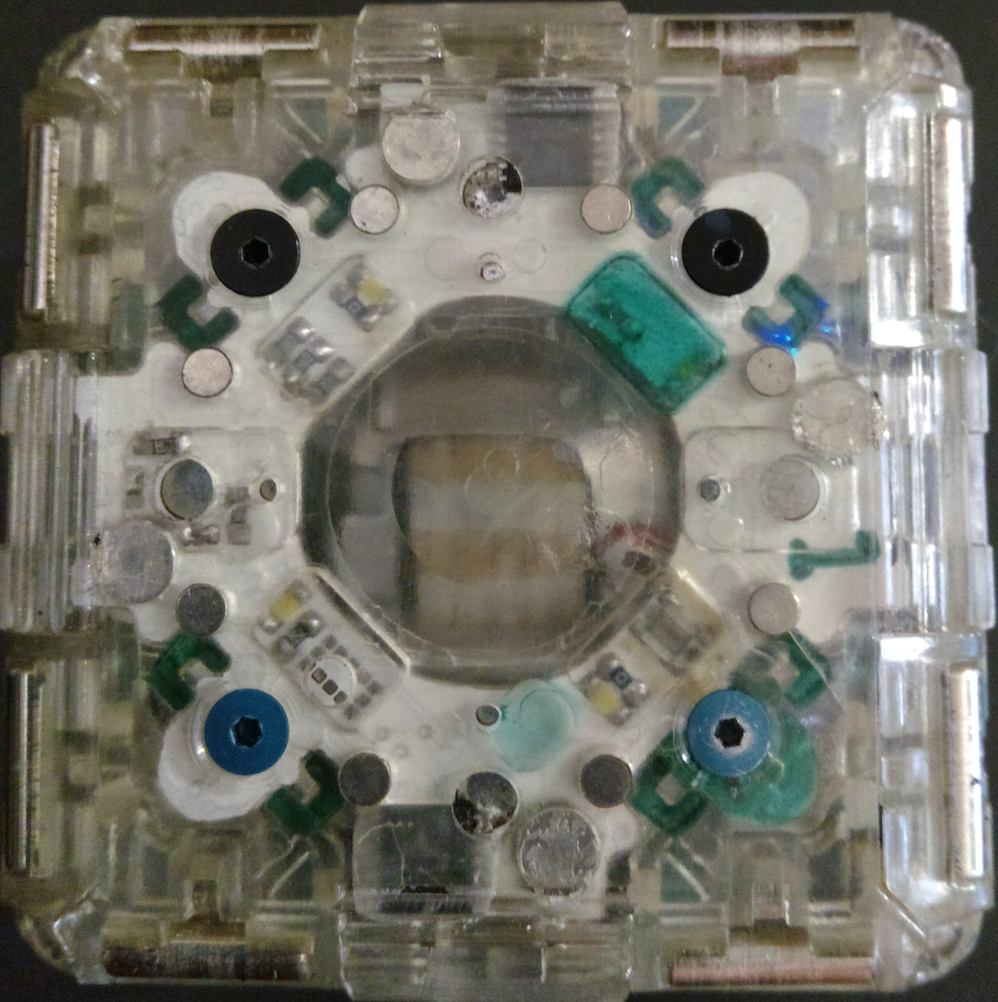
\includegraphics[width = 5.9 cm]{figures/face.png}};
	\node at (3 cm, 3 cm) {\usebox{\faceDiagram}};
	\node at (10 cm, 3 cm) {\usebox{\magnetDigitization}};
	\node at (15.5 cm, 2cm) {\usebox{\gridFigure}};
	
	%\node[fill=orange] at (3,3) {\textbf{18}};
	
	\tikzmath{
		\smallBoxX = 0.5;
		\smallBoxY = 2.9;
	}

	% Small Box around Magnet
	%\node[draw, purple, dotted, minimum size = 1.25 cm, rounded corners, thick] at (3.65cm , 7cm) {};
	
	\path[draw, purple, dotted, minimum size = 1.25 cm, rounded corners, ultra thick]
	(3*0.7, 6.25*0.7) --
	++(1.25, 0) --
	++(0, 1.25) --
	++(-1.25, 0) --
	cycle {};
	
	\node (a) at (12.5, 3){};
	\node (b) at (14.75, 3.4){};
	
	\draw[>={Stealth[round]}, purple,dashed, ultra thick, bend right, rounded corners = 1 cm, ->] (a) -- (13.75,5) -- (b);
	
	\draw[purple,dashed, thin] (2.7cm, 4.35cm + 1.25cm) -- ++(358: 4.8cm);
	\draw[purple,dashed, thin] (2.7cm, 4.35cm ) -- ++(323: 5.9cm);
	
	% Large Purple box
	\node[draw, purple, dotted, minimum size = 5 cm, rounded corners,ultra thick] at (10cm , 3cm) {};
	
	\node[] at (10cm , 0.2cm) {Discretizing Angle};
	%\draw (1,1) pic {complexnode} (4,4);
	
	\end{tikzpicture}
	
	
	
	
%	\newsavebox{\faceDiagram}
%	\sbox{\faceDiagram}	{
%		\newcommand{\statcirc}[4]{
	\fill[opacity = 0.5, red,shift={(#1 cm,#2 cm)}, rotate=#3] (0,0) circle (#4); 
	\fill[opacity = 0.5, blue,shift={(#1 cm,#2 cm)},rotate=#3] (0,0) -- (180:#4) arc (180:0:#4) -- cycle;
	%	\draw[->,black,shift={(#1 cm,#2 cm)},rotate=#3] (#4, 0)
}

\newcommand{\drawArrow}[3]{
	\draw[->,>={Stealth[round]}, line width=0.75mm, black ,shift={(#1 cm,#2 cm)}, rotate=#3] (0,-0.5) -- (0,0.5); 
}

\newcommand{\drawchip}[3]{
	\tikzmath
	{
		\chipW = 0.35;
		\chipH = 0.4;
	}
	\fill[opacity = 0.75, darkgray, shift= {(#1 cm, #2 cm)}, rotate = #3, rounded corners] (-\chipH,-\chipW) rectangle (\chipH,\chipW);
	\fill[orange,shift= {(#1 cm, #2 cm)}, rotate = #3 ] (-0.25,0.2) circle (0.1);
}
\begin{tikzpicture}

	\tikzmath{
		\offsetAxis = 0.5;
		\offsetCent = 2.9;
		\diameter = 0.32;
	}
	\draw node (A) at (-0.5, 1.7) {};
	\draw node (B) at (0, 1.7) {};
	\drawchip{\offsetAxis}{\offsetCent}{0};
	\drawchip{-\offsetAxis}{-\offsetCent}{180};
	
	%Magnet North
	\statcirc{-\offsetAxis}{\offsetCent}{70}{\diameter};
	
	\drawArrow{-\offsetAxis}{\offsetCent}{70}
	
	%Magnet EAST
	\statcirc{\offsetCent}{\offsetAxis}{20}{\diameter};
	
	% Magnet West
	\statcirc{\offsetAxis}{-\offsetCent}{190}{\diameter};
	
	\statcirc{-\offsetCent}{-\offsetAxis}{45}{\diameter};
	
	\draw[gray, dashed] (-\offsetAxis,{\offsetCent + 1}) -- 
	(-\offsetAxis,{\offsetCent - 1});
	\draw[black,dotted] (0,0) circle (2.95);
	
	% 4 Cross Lines X
	\draw[black,dashed] (0,0) -- (4,0);
	\draw[black,dashed] (0,0) -- (-4,0);
	\draw[black,dashed] (0,0) -- (0,4);
	\draw[black,dashed] (0,0) -- (0,-4);
	
%	\draw[purple, dotted] ()
	% Dimensioned Variables
	\dimline[line style = {line width = 0.8, arrows = dimline reverse-dimline reverse}] {(A)}{(B)}{x};
	
	% Arc Radius
	\dimline[line style = {line width = 0.8}] {(0,0)} {++(150:2.95)}{R};
%	\dimline {(1,0)}{(-1,0)}{x};
\end{tikzpicture}
%	}
%	
%	\newsavebox{\magnetDigitization}
%	\sbox{\magnetDigitization}	{
%		
\newcommand{\statcirc}[4]{
	\fill[red,shift={(#1 cm,#2 cm)}, rotate=#3] (0,0) circle (#4); 
	\fill[blue,shift={(#1 cm,#2 cm)},rotate=#3] (0,0) -- (180:#4) arc (180:0:#4) -- cycle;
	%	\draw[->,black,shift={(#1 cm,#2 cm)},rotate=#3] (#4, 0)
}

\newcommand{\drawArrow}[3]{
	\draw[->,>={Stealth[round]}, line width=0.75mm, black ,shift={(#1 cm,#2 cm)}, rotate=#3] (0,-1) -- (0,1); 
}

\begin{tikzpicture}[scale = 0.75]
\tikzmath{
	\offsetAxis = 0.5;
	\offsetCent = 2.9;
	\diameter = 0.75;
}

\foreach \i in {1,...,30}
{
	\draw[gray] (0,0) -- (\i * 12-6 : 2.8);
	\node[inner sep=0pt] at (-{\i * 12}+12: 3) {\i};
}
\node[circle,draw,inner sep=0pt, fill = green] at (-{18 * 12}+12: 3) {18};
\statcirc{0}{0}{-204-90}{\diameter};
\drawArrow{0}{0}{-204-90};
\draw[black,dashed] (0,0) -- (3,0);
\draw[black,dashed] (0,0) -- (-3,0);
\draw[black,dashed] (0,0) -- (0,3);
\draw[black,dashed] (0,0) -- (0,-3);
\draw[gray, dotted] (0,0) -- (-204: 3);
\draw[gray, dotted] (0,0) -- (-204: 3);
\draw [white, line width = 5pt] (2.1,0)  arc (0:360-204:2.1);
\draw [<->, >={Stealth[round]}] (2.1,0)  arc (0:360-204:2.1);
\node[circle,inner sep=3pt, fill = white]				at (90:2) {$\theta$};
\end{tikzpicture}
%	}
%	
%	\newsavebox{\gridFigure}
%	\sbox{\gridFigure}	{
%		\begin{tikzpicture}[every node/.style={minimum size=2 cm-\pgflinewidth, outer sep=0pt}]
    \draw[step=2cm,color=black] (0,0) grid (4,4);

    \node[fill=orange] at (+1,+1) {};
   % \node[fill=yellow] at (+0.75,+0.75) {};
\end{tikzpicture}
%	}
%	%\begin{tikzpicture}[minimum width = 14 cm, minimum height = 6 cm]
%	%\draw (0,0) -- (14,6);
%	
%	\begin{tikzpicture}[]
%	%complexnode/.pic={\usebox{\mybox}}]
%	
%	\newcommand\xa{2};
%	\newcommand\xb{2};
%	\newcommand\ya{2};
%	\newcommand\yb{2};
%	
%	\coordinate (smallNE) at (2,5);
%	\coordinate (smallSE) at (2,5);
%	\coordinate (smallSW) at (2,5);
%	\coordinate (smallNW) at (2,5);
%	
%	\coordinate (bigNE) at (2,5);
%	\coordinate (bigSE) at (2,5);
%	\coordinate (bigSW) at (2,5);
%	\coordinate (bigSE) at (2,5);
%	
%	\node[opacity = 0.95] at (4.25 cm, 4 cm) {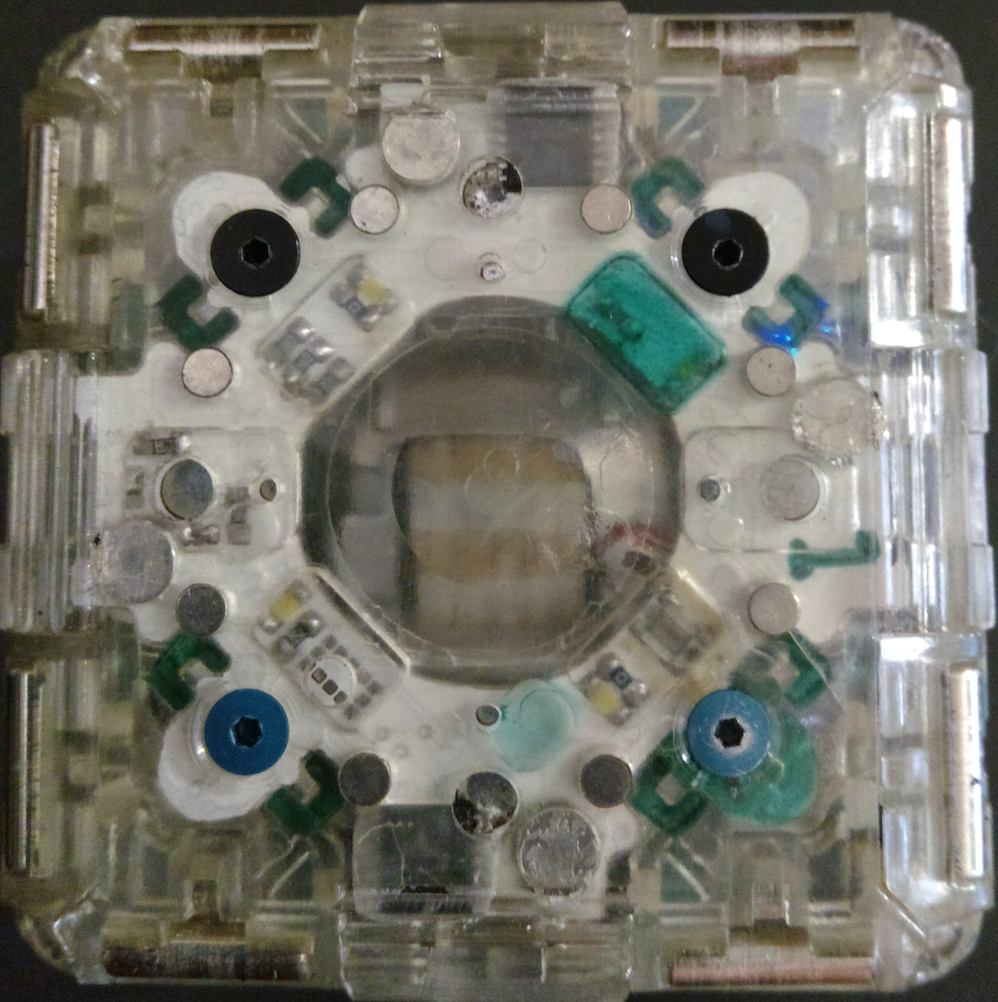
\includegraphics[width = 8 cm]{figures/face.png}};
%	\node at (4 cm, 4 cm) {\usebox{\faceDiagram}};
%	\node at (11 cm, 6 cm) {\usebox{\magnetDigitization}};
%	\node at (15 cm, 2cm) {\usebox{\gridFigure}};
%	
%	%\node[fill=orange] at (3,3) {\textbf{18}};
%	
%	\tikzmath{
%		\smallBoxX = 0.5;
%		\smallBoxY = 2.9;
%	}
%	
%	% Small Box around Magnet
%	%\node[draw, purple, dotted, minimum size = 1.25 cm, rounded corners, thick] at (3.65cm , 7cm) {};
%	
%	\path[draw, purple, dotted, minimum size = 1.25 cm, rounded corners, ultra thick]
%	(3, 6.25) --
%	++(1.25, 0) --
%	++(0, 1.25) --
%	++(-1.25, 0) --
%	cycle {};
%	
%	\node (a) at (13.5, 6){};
%	\node (b) at (15.75, 3.5){};
%	\draw[>={Stealth[round]}, purple,dashed, ultra thick, bend right, rounded corners = 1 cm, ->] (a) -- (15.75,6) -- (b);
%	\draw[purple,dashed, thin] (3.5cm, 6.25cm + 1.25cm) -- ++(10: 5cm);
%	\draw[purple,dashed, thin] (3.5cm, 6.25cm ) -- ++(332: 5.45cm);
%	
%	% Large Purple box
%	\node[draw, purple, dotted, minimum size = 4.8 cm, rounded corners,ultra thick] at (11cm , 6cm) {};
%	
%	%\draw (1,1) pic {complexnode} (4,4);
%	
%	\end{tikzpicture}
	
	\caption{Figure illustrating the \TagNamePlural~ system. A tag consists of four permanent magnets placed according to two dimensions, (R) is the circle diameter, and (x) is the offset from the y axis. The left half shows a photo of one of the m-blocks superimposed with the magnets and sensors. The absolute angle of the magnet, relative to a line extending from the center of the face is then digitized by an absolute magnetic encoder (black rectangle with orange dot).}
	\label{fig:tagDiagram}
\end{figure*}

%%%%%%%%%%%%%%%%%%%%%%%%%%%%%%%%%%%%%%%%%%%%%%%%%%%%%%%%%%%%%%%%%%%%%%%%%%%%%%%%%%%%%%%%%%%%%%%%%%%%%%%%%%%%%%%%%%%%%%%%%%%%%%%%%%%%%%%%%%%%%%%
%%%%%%%%%%%%%%%%%%%%%%%%%%%%%%%%%%%%%%%%%%%%%%%%%%%%%%%%%%%%%%%%%%%%%%%%%%%%%%%%%%%%%%%%%%%%%%%%%%%%%%%%%%%%%%%%%%%%%%%%%%%%%%%%%%%%%%%%%%%%%%%
%\subsection{\tagNamePlural Characterization}
%\label{sec:tagsCharacterize}
%%%%%%%%%%%%%%%%%%%%%%%%%%%%%%%%%%%%%%%%%%%%%%%%%%%%%%%%%%%%%%%%%%%%%%%%%%%%%%%%%%%%%%%%%%%%%%%%%%%%%%%%%%%%%%%%%%%%%%%%%%%%%%%%%%%%%%%%%%%%%%%
%%%%%%%%%%%%%%%%%%%%%%%%%%%%%%%%%%%%%%%%%%%%%%%%%%%%%%%%%%%%%%%%%%%%%%%%%%%%%%%%%%%%%%%%%%%%%%%%%%%%%%%%%%%%%%%%%%%%%%%%%%%%%%%%%%%%%%%%%%%%%%%

While the exact performance of the \tagName~system that will be be implementation dependant i.e. different size/shape magnets, sensor ICs, etc. We performed an experiment shown in Figure~\ref{fig:histogram} to demonstrate that our implementation of the \tagName~concept is feasible and useful in the context of modular robots. While the angular resolution of the magnetic angular encoders that we used is very high, 14 bits for the AS5048b used in this work, these readings are only repeatable under ideal conditions. There are many factors which influence the accuracy of readings of the sensors in the context of the \tagNamePlural. We have identified the following factors that contribute to reading errors: (1) relative alignment of the face containing the tag to the face containing the reader. (2) alignment of the magnetic sensor relative to the face of the module. (3) variability of the magnetic field direction in the manufacture of the magnets. (4) mechanical alignment of the magnets in reference to the tag. (5) effects of external magnetic fields. While factors 2 and 4 appear to be a significant factor in the errors seen in this system, we think that much of this error is due to the inaccurate hand-assembled nature of this prototype system.

\begin{figure}[h]
	% Data

\begin{tikzpicture}
\begin{axis}[
height=4cm,
width=9cm,
%            ybar interval,      % <-- this causes the `xticks' to be centered
ymin= 0, ymax=5,
xmin=-11, xmax=11,
grid=both,
minor y tick num=1,
%yminorgrids=true,
tick align=outside, % <-- this positions the ticks "outside"
]
\addplot+ [
ybar interval,
mark=none,
fill=blue!25,   % fill the bars again
] coordinates {

	(-10,0)	%
	(-9,0)	%
	(-8,0)	%
	(-7,1)	%
	(-6,0)	%1
	(-5,1)	%11
	(-4,1)	%11
	(-3,1)	%111111
	(-2,2)	%11111
	(-1,3)	%111111
	 (0,4)	%11111
	 (1,3)	%1
	 (2,5)	%
	 (3,4)	%
	 (4,3)	%
	 (5,1)	%
	 (6,1)	%
	 (7,1)	%
	 (8,0)	%
	 (9,0)	%
	 (10,1)	%

};

\addplot+ [
ybar interval,
mark=none,
fill=black,   % fill the bars again
] coordinates {
	(-6.05,16) 
	(-5.95,16) 
};

\addplot+ [
ybar interval,
mark=none,
fill=black,   % fill the bars again
] coordinates {
	(6.05,16) 
	(5.95,16) 
};
\end{axis}

\end{tikzpicture}
	\caption{Histogram showing one sensor face reading the same tag multiple times. The Boundary lines represents tags that will were mis-read. In this case about 9\% of the tags were misread - but this can be solved by assigning several adjacent digits to the same tag to dramatically improve the accuracy, and should be reduced with more repeatable manufacturing methods.}
	\label{fig:histogram}
\end{figure}


%%%%%%%%%%%%%%%%%%%%%%%%%%%%%%%%%%%%%%%%%%%%%%%%%%%%%%%%%%%%%%%%%%%%%%%%%%%%%%%%%%%%%%%%%%%%%%%%%%%%%%%%%%%%%%%%%%%%%%%%%%%%%%%%%%%%%%%%%%%%%%
%%%%%%%%%%%%%%%%%%%%%%%%%%%%%%%%%%%%%%%%%%%%%%%%%%%%%%%%%%%%%%%%%%%%%%%%%%%%%%%%%%%%%%%%%%%%%%%%%%%%%%%%%%%%%%%%%%%%%%%%%%%%%%%%%%%%%%%%%%%%%%
%\begin{figure}[h]
%	\begin{tikzpicture}
\begin{axis}[view={-20}{20}, grid=both]
\addplot3[surf] file {data.txt};
\end{axis}
\end{tikzpicture}
       
%	\caption{Figure showing the error in the reading from a reader reading a tag as it is moved in X and Y relative to perfect alignment.}
%	\label{fig:histogram}
%\end{figure}
%%%%%%%%%%%%%%%%%%%%%%%%%%%%%%%%%%%%%%%%%%%%%%%%%%%%%%%%%%%%%%%%%%%%%%%%%%%%%%%%%%%%%%%%%%%%%%%%%%%%%%%%%%%%%%%%%%%%%%%%%%%%%%%%%%%%%%%%%%%%%%
%%%%%%%%%%%%%%%%%%%%%%%%%%%%%%%%%%%%%%%%%%%%%%%%%%%%%%%%%%%%%%%%%%%%%%%%%%%%%%%%%%%%%%%%%%%%%%%%%%%%%%%%%%%%%%%%%%%%%%%%%%%%%%%%%%%%%%%%%%%%%%